\documentclass[12pt, twoside,a4paper, landscape]{article}
\oddsidemargin = 10pt
\textwidth = 430pt

\usepackage{fullpage}	 %to make smaller margins
\usepackage{graphicx}
%\usepackage[utf8]{inputenc}
%\usepackage[T1]{fontenc}
%\usepackage{url}

\usepackage[hidelinks]{hyperref}
\usepackage{pdfpages}
\usepackage{placeins}
\usepackage{graphicx}
\usepackage[font=small,labelfont=bf]{caption}
\usepackage{subfig}

%\usepackage{subcaption}
\usepackage{enumerate}
\usepackage{amsmath}
\usepackage{listings} %for showing program code
\usepackage{bm}
\usepackage{wrapfig}
\usepackage{lipsum}
\usepackage{float}
\usepackage{titlesec}	
\usepackage{amsfonts}
\usepackage{amssymb}
\usepackage[comma,authoryear]{natbib}
\usepackage{epstopdf}


%\titlespacing*{\chapter}{0pt}{-10pt}{20pt}
%\titleformat{\chapter}[display]{\normalfont\huge\bfseries}{}{35pt}{}

\setlength{\intextsep}{0pt} %to make wrapfigures beautiful
%\setlength{\oddsidemargin}{0.5cm}
%\setlength{\evensidemargin}{-0.5cm}
\begin{document}
Given the general rendering equation
$$
L_o(x_o, \vec{\omega}_o) = L_e(x_o, \vec{\omega}_o) + L_r(x_o, \vec{\omega}_o)  
$$
$$
L_o(x_o, \vec{\omega}_o) = L_e(x_o, \vec{\omega}_o) + \int_A \int_{2 \pi} S(x_i, \vec{\omega}_i, x_o, \vec{\omega}_o) L_i(x_i, \vec{\omega}_i) (\vec{\omega}_i \cdot \vec{n}_i) d \vec{\omega}_i dA 
$$

The inner integarl can be eliminated if we consider only one directional light source. That leads to the following equation:

$$
L_o(x_o, \vec{\omega}_o) = \sum_{i = 0}^{N} S(x_i, \vec{\omega}_d, x_o, \vec{\omega}_o)\; (\vec{\omega}_d \cdot \vec{n}_i) \; V(n_i,\vec{\omega}_d) \;L_d \;A_i 
$$
Where $A_i$ is the barycentric area (sum of vertex to the neighboring triangles to closest barycenter), N is the number of vertices of the mesh, and $\vec{\omega}_d$, $L_d$ are the direction towards and the radiance of a directional light. $V(n_i,\vec{\omega}_d)$ is a visibility function defined as follows:

\begin{equation}
V(n_i,\vec{\omega}_d) = \begin{cases} 1 &\mbox{if } \vec{\omega}_d \cdot \vec{n}_i > 0 \\ 
0 & \mbox{otherwise } \end{cases} 
\end{equation}

That holds for the simple models used.

As we can see from the following results, there it seems to be a slight overshoot on the directional dipole model: needs investigation.


\begin{figure}[here]
\centering
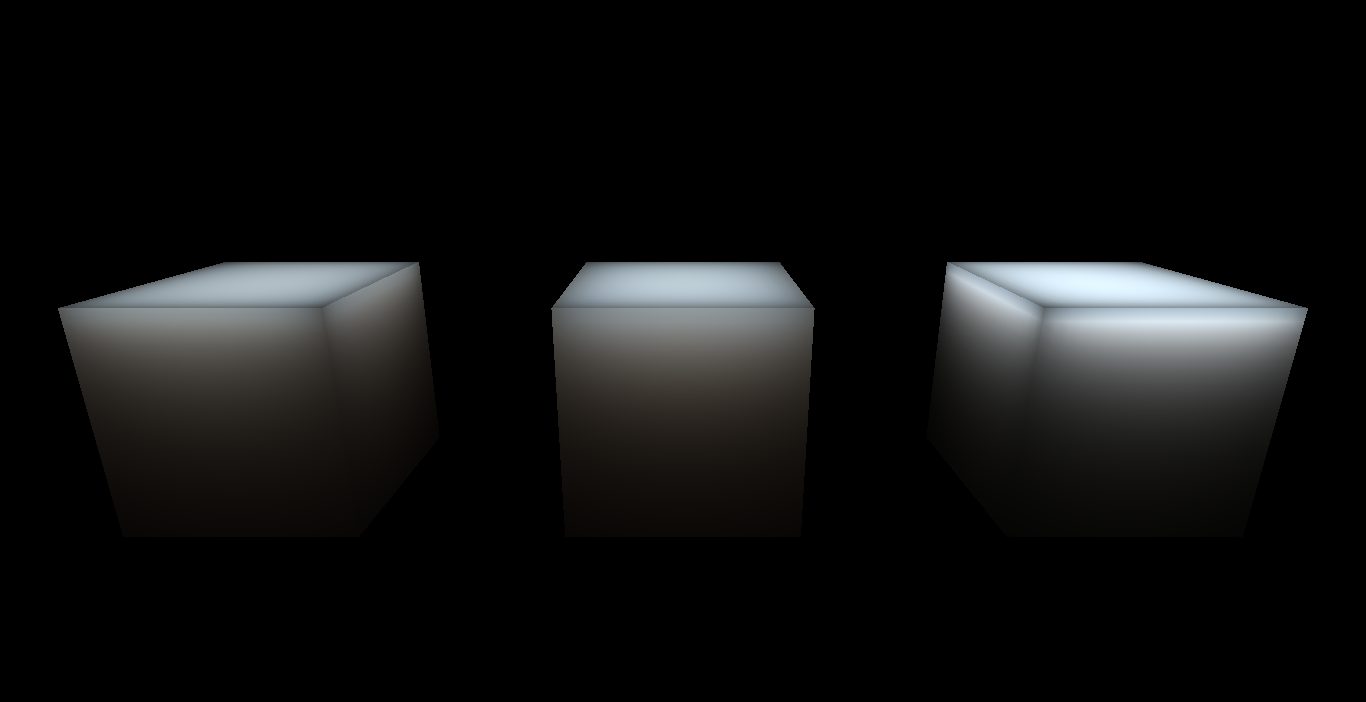
\includegraphics[width=0.8\textwidth]{marblecubes}
\caption{Marble set of cubes. Left to right: Jensen et al. dipole, D'Eon et al. better dipole and Frisvad et al. directional dipole. Material properties for marble.}
\end{figure}

\begin{figure}[here]
\centering
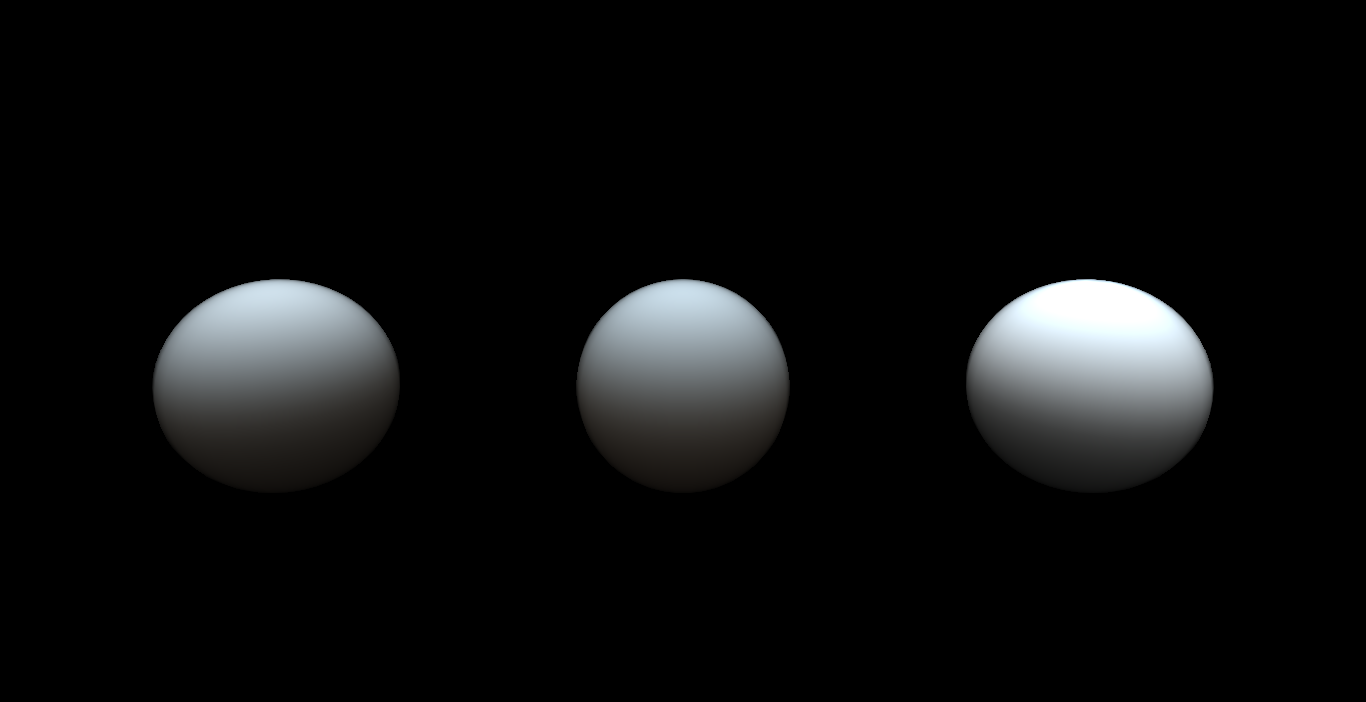
\includegraphics[width=0.8\textwidth]{marblespheres}
\caption{Marble set of spheres. Left to right: Jensen et al. dipole, D'Eon et al. better dipole and Frisvad et al. directional dipole. Material properties for marble.}
\end{figure}

\begin{figure}[here]
\centering
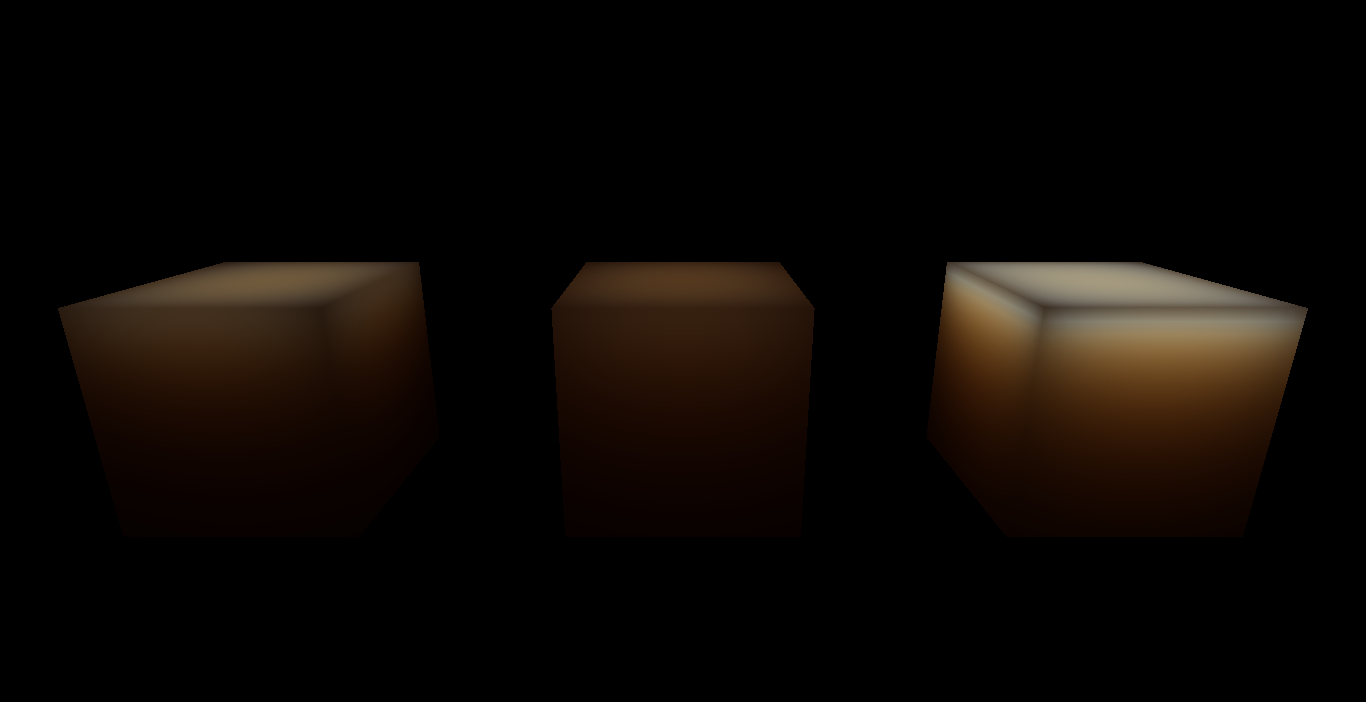
\includegraphics[width=0.8\textwidth]{chocolatecubes}
\caption{Regular chocolate milk set of cubes. Left to right: Jensen et al. dipole, D'Eon et al. better dipole and Frisvad et al. directional dipole. Material properties for regular chocolate milk.}
\end{figure}

\begin{figure}[here]
\centering
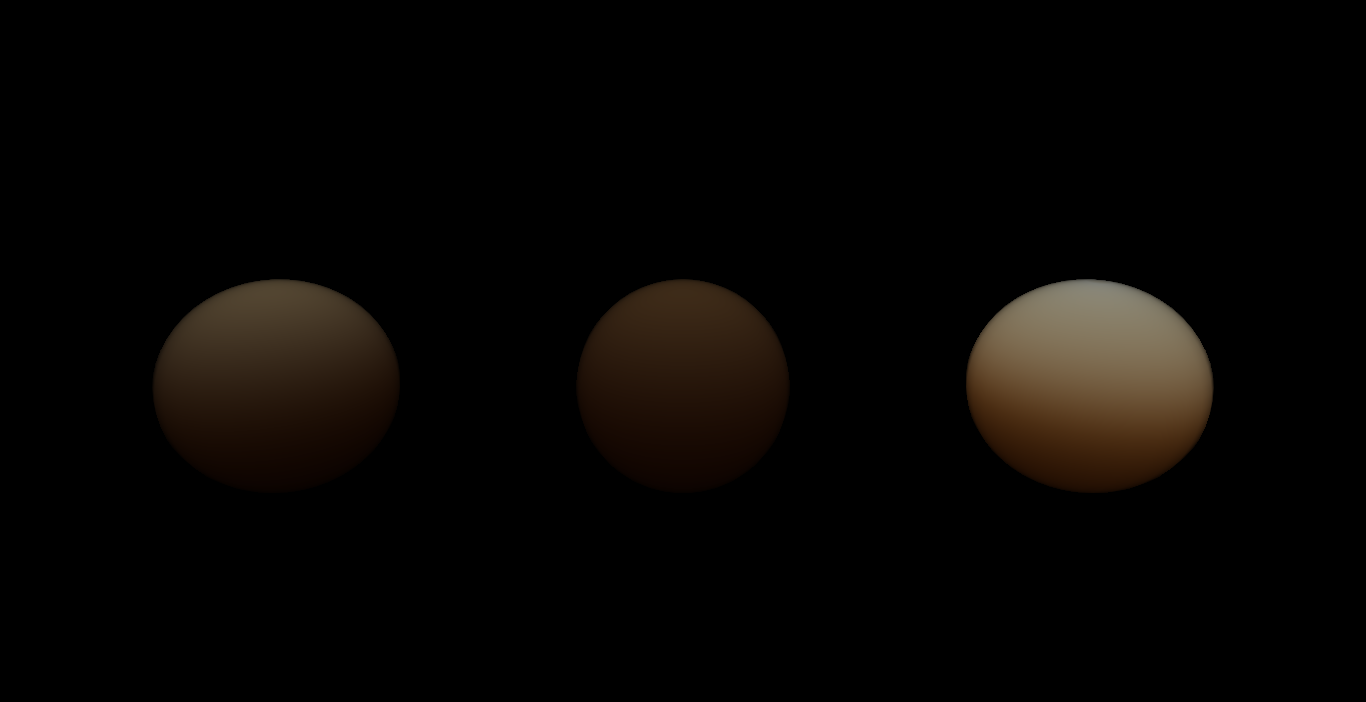
\includegraphics[width=0.8\textwidth]{chocolatespheres}
\caption{Regular chocolate milk set of spheres. Left to right: Jensen et al. dipole, D'Eon et al. better dipole and Frisvad et al. directional dipole. Material properties for regular chocolate milk.}
\end{figure}


\begin{figure}[here]
\centering
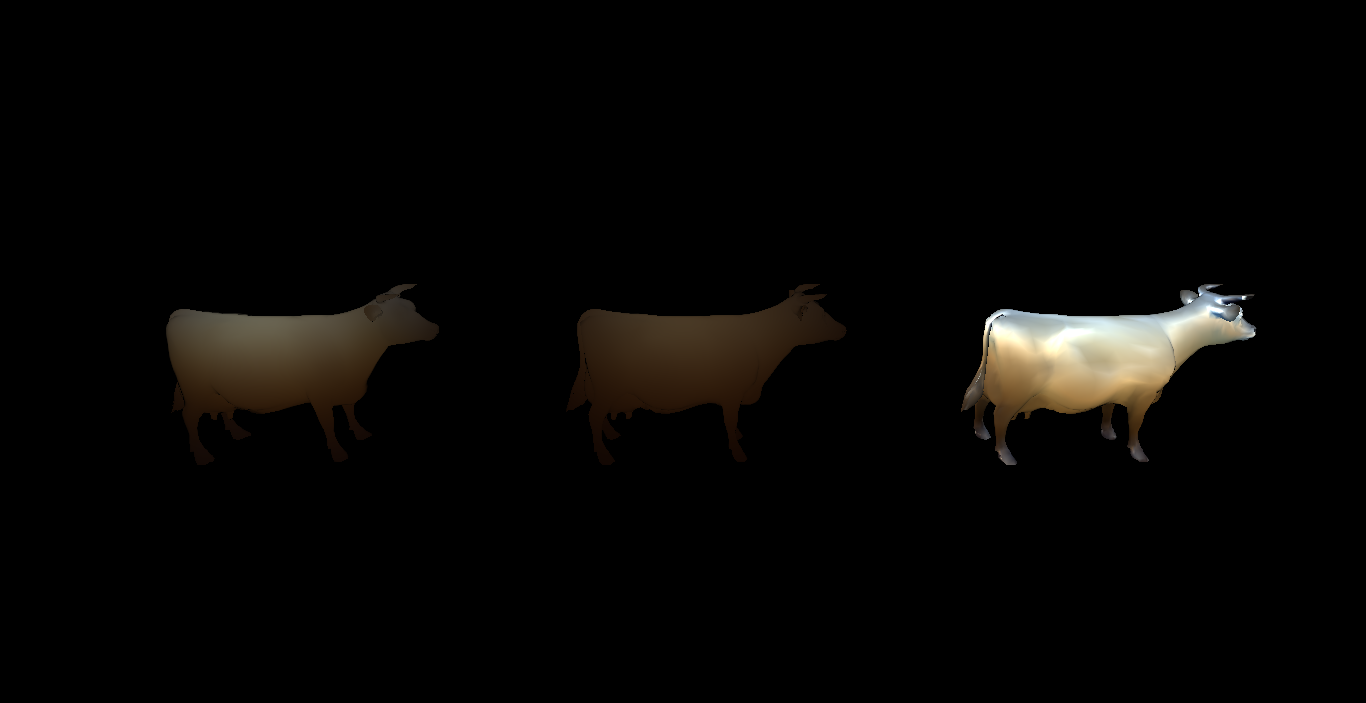
\includegraphics[width=0.8\textwidth]{cowmilk}
\caption{Regular chocolate milk set of cow. Left to right: Jensen et al. dipole, D'Eon et al. better dipole and Frisvad et al. directional dipole. Material properties for regular chocolate milk.}
\end{figure}

\end{document}
